\section{\K 集成运算放大器的基本知识}
\Par 集成运算放大器对于我们来说相当于一个黑箱,它主要由输入级、输出级、中间级和偏置电路组成.集成电路能实现放大的功能,并且放大倍数很高.其中输入端标记有“-”号的称为反向端,标记有“+”号的称为正向端,反向端输入的电压与输出电压反相(相位相差$\pi$),正向端输入的电压与输出电压同相.
\begin{figure}[htbp]
	\centering
	\begin{minipage}[b]{0.48\textwidth}
        \centering
        \includegraphics[width=0.65\textwidth]{集成运算放大器组成图.jpg}
        \caption{集成运算放大器组成图}
	    \label{fig:集成运算放大器组成图}
    \end{minipage}
    \begin{minipage}[b]{0.48\textwidth}
        \centering
        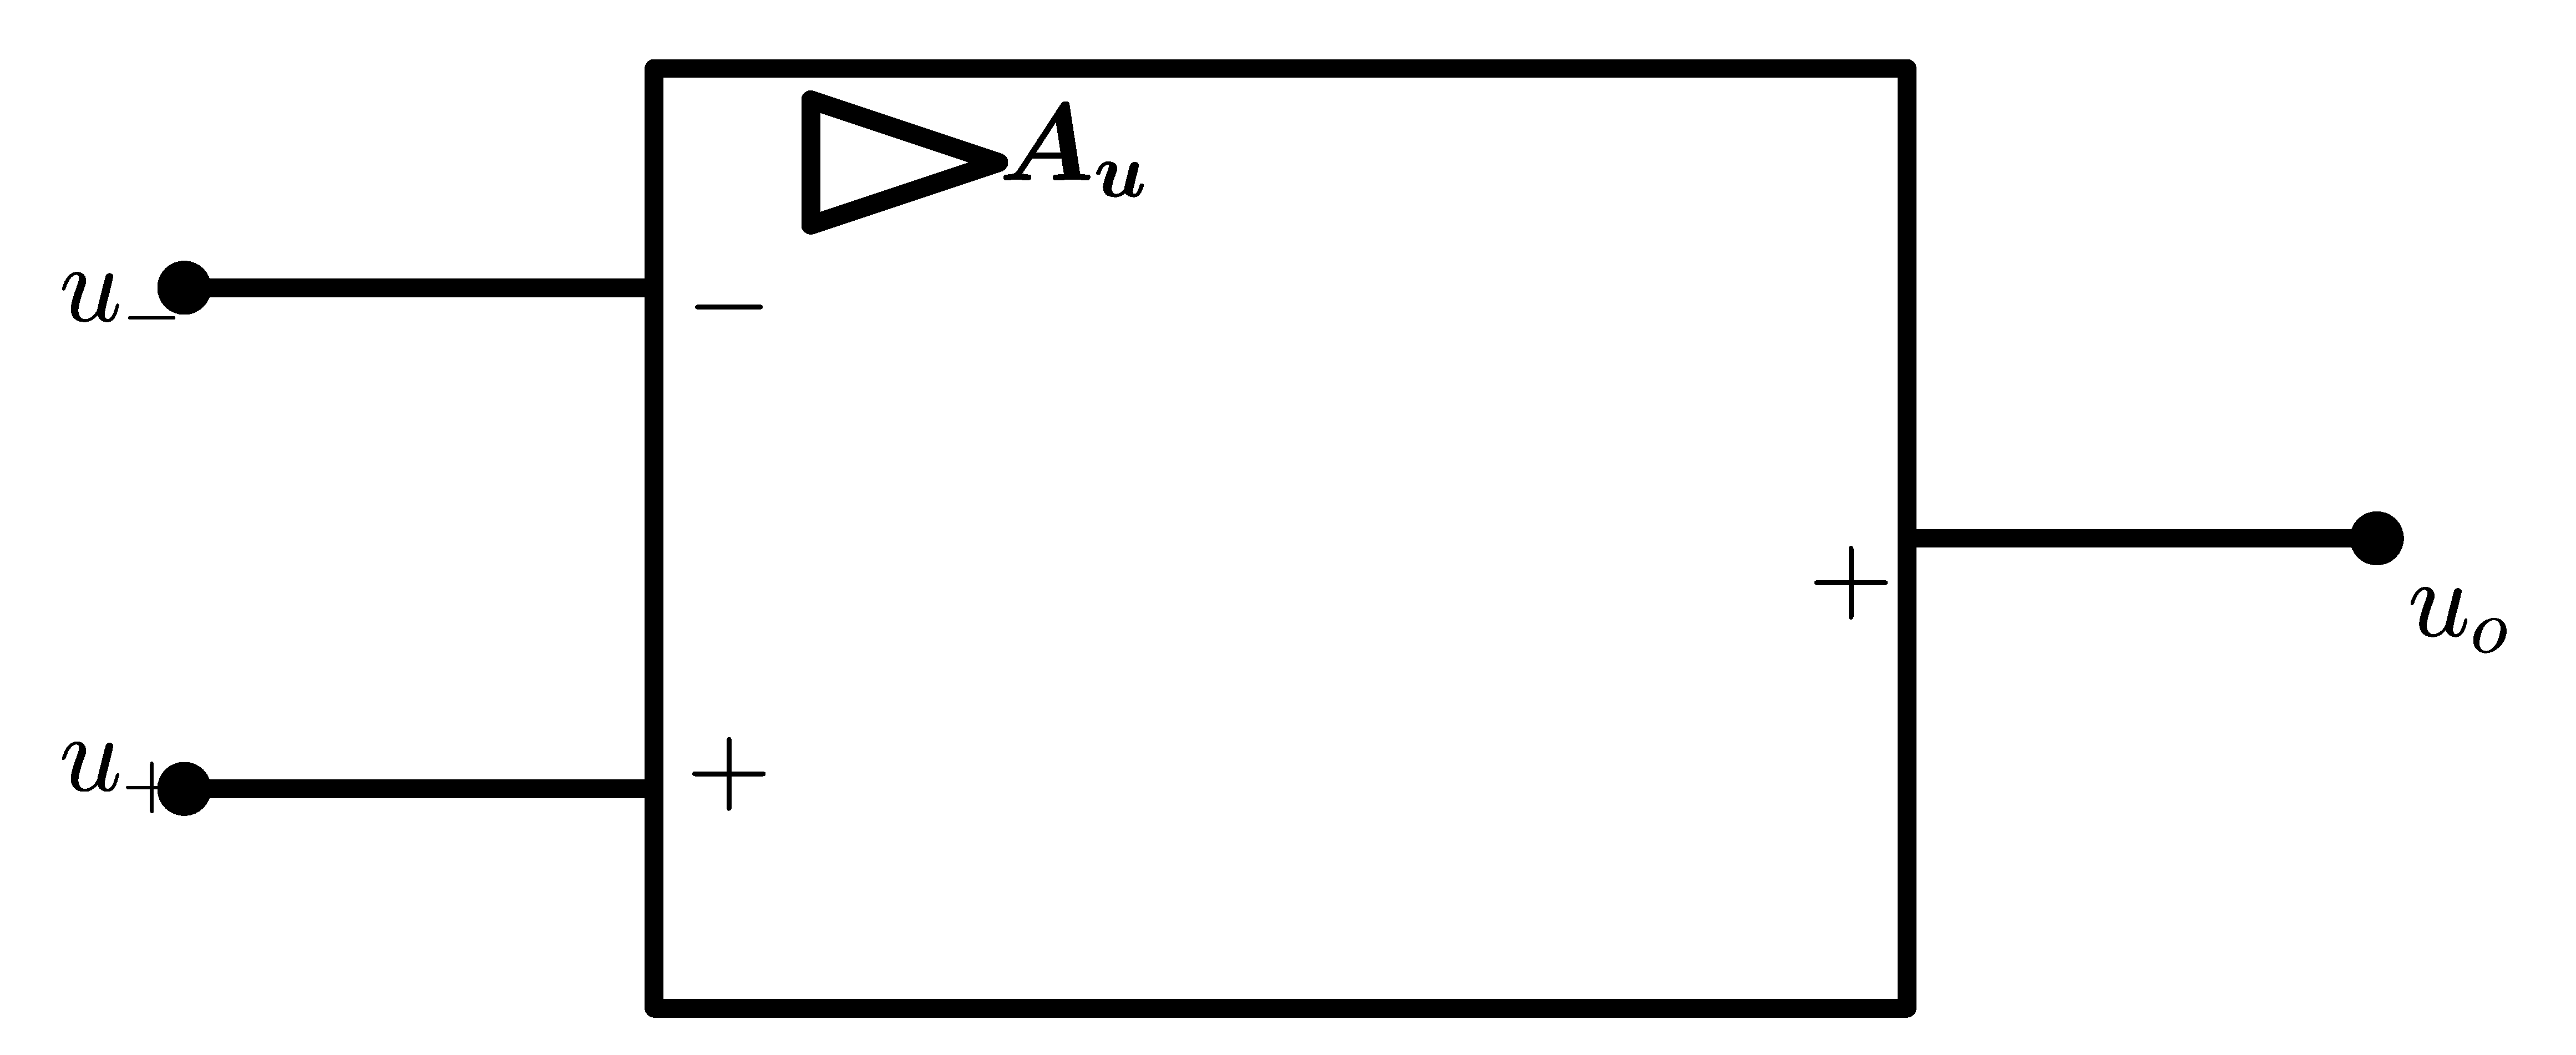
\includegraphics[width=0.65\textwidth]{集成运算放大器的符号.pdf}
        \caption{集成运算放大器的符号}
	    \label{fig:集成运算放大器的符号}
    \end{minipage}
\end{figure}

\Par 以下是它的基本参数
\begin{equation*}
    \begin{matrix}
        \mathrm{A}_{\mathrm{uo}}&		\text{高}:80\mathrm{dB}\sim 140\mathrm{dB}\\
        \mathrm{r}_{\mathrm{id}}&		\text{高}:10^5\sim 10^{11}\\
        \mathrm{r}_{\mathrm{o}}&		\text{低}:\text{几十}\Omega \sim \text{几百}\Omega\\
        \mathrm{K}_{\mathrm{CMR}}&		\text{高}:70\mathrm{dB}\sim 130\mathrm{dB}\\
    \end{matrix}
\end{equation*}
\Par 如图\ref{fig:电压传输特性}所示,由于集成电路的放大效果太好,导致它很容易就进入饱和区,使得输出电压到达峰值,为此我们可以设置一个负反馈装置来抑制它的增大.图中$U_{im}$表示最大输入电压,$U_{o(sat)}$表示最大输出电压.

\begin{figure}[htbp]
	\centering
	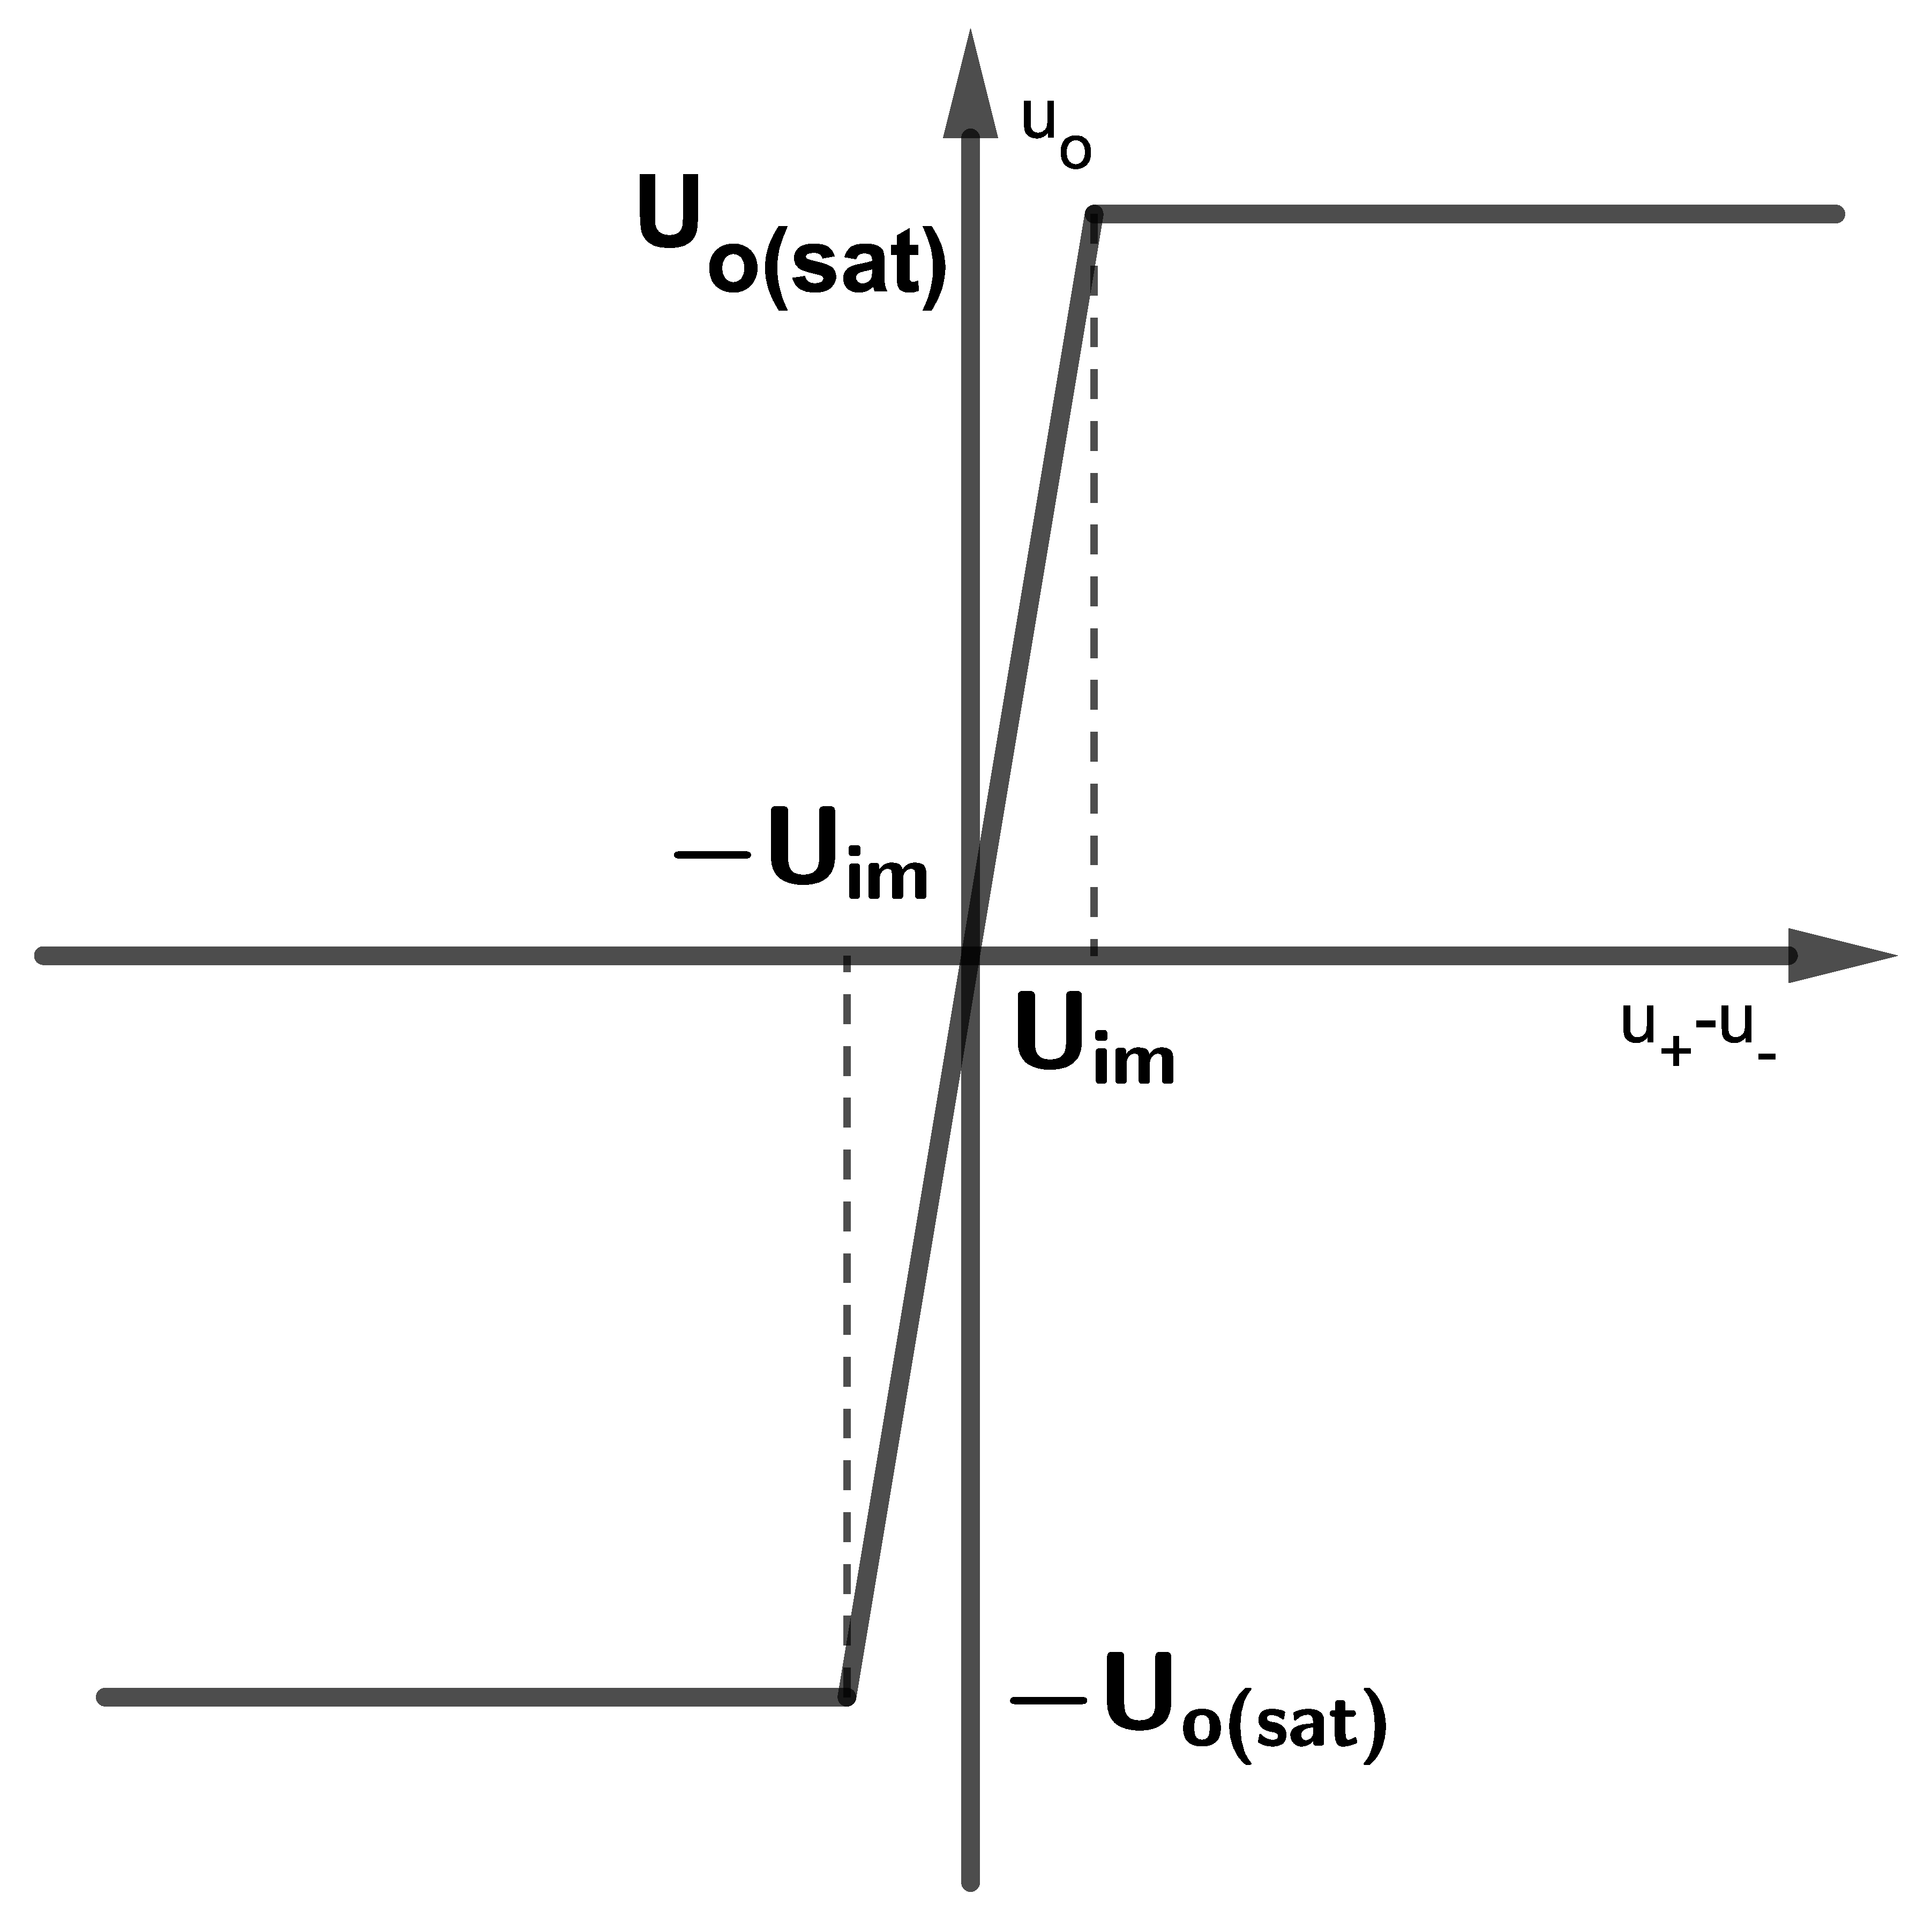
\includegraphics[width=0.35\textwidth]{电压传输特性.pdf}
	\caption{电压传输特性}
	\label{fig:电压传输特性}
\end{figure}

\Par 为了进一步讨论,我们将集成运算放大器拓展成理想集成运算放大器,它的参数满足
\begin{equation*}
    \begin{matrix}{l}
        \mathrm{A}_{\mathrm{uo}}&		+\infty\\
        \mathrm{r}_{\mathrm{id}}&		+\infty\\
        \mathrm{r}_{\mathrm{o}}&		0\\
        \mathrm{K}_{\mathrm{CMR}}&		+\infty\\
    \end{matrix}
\end{equation*}
\begin{figure}[htbp]
	\centering
	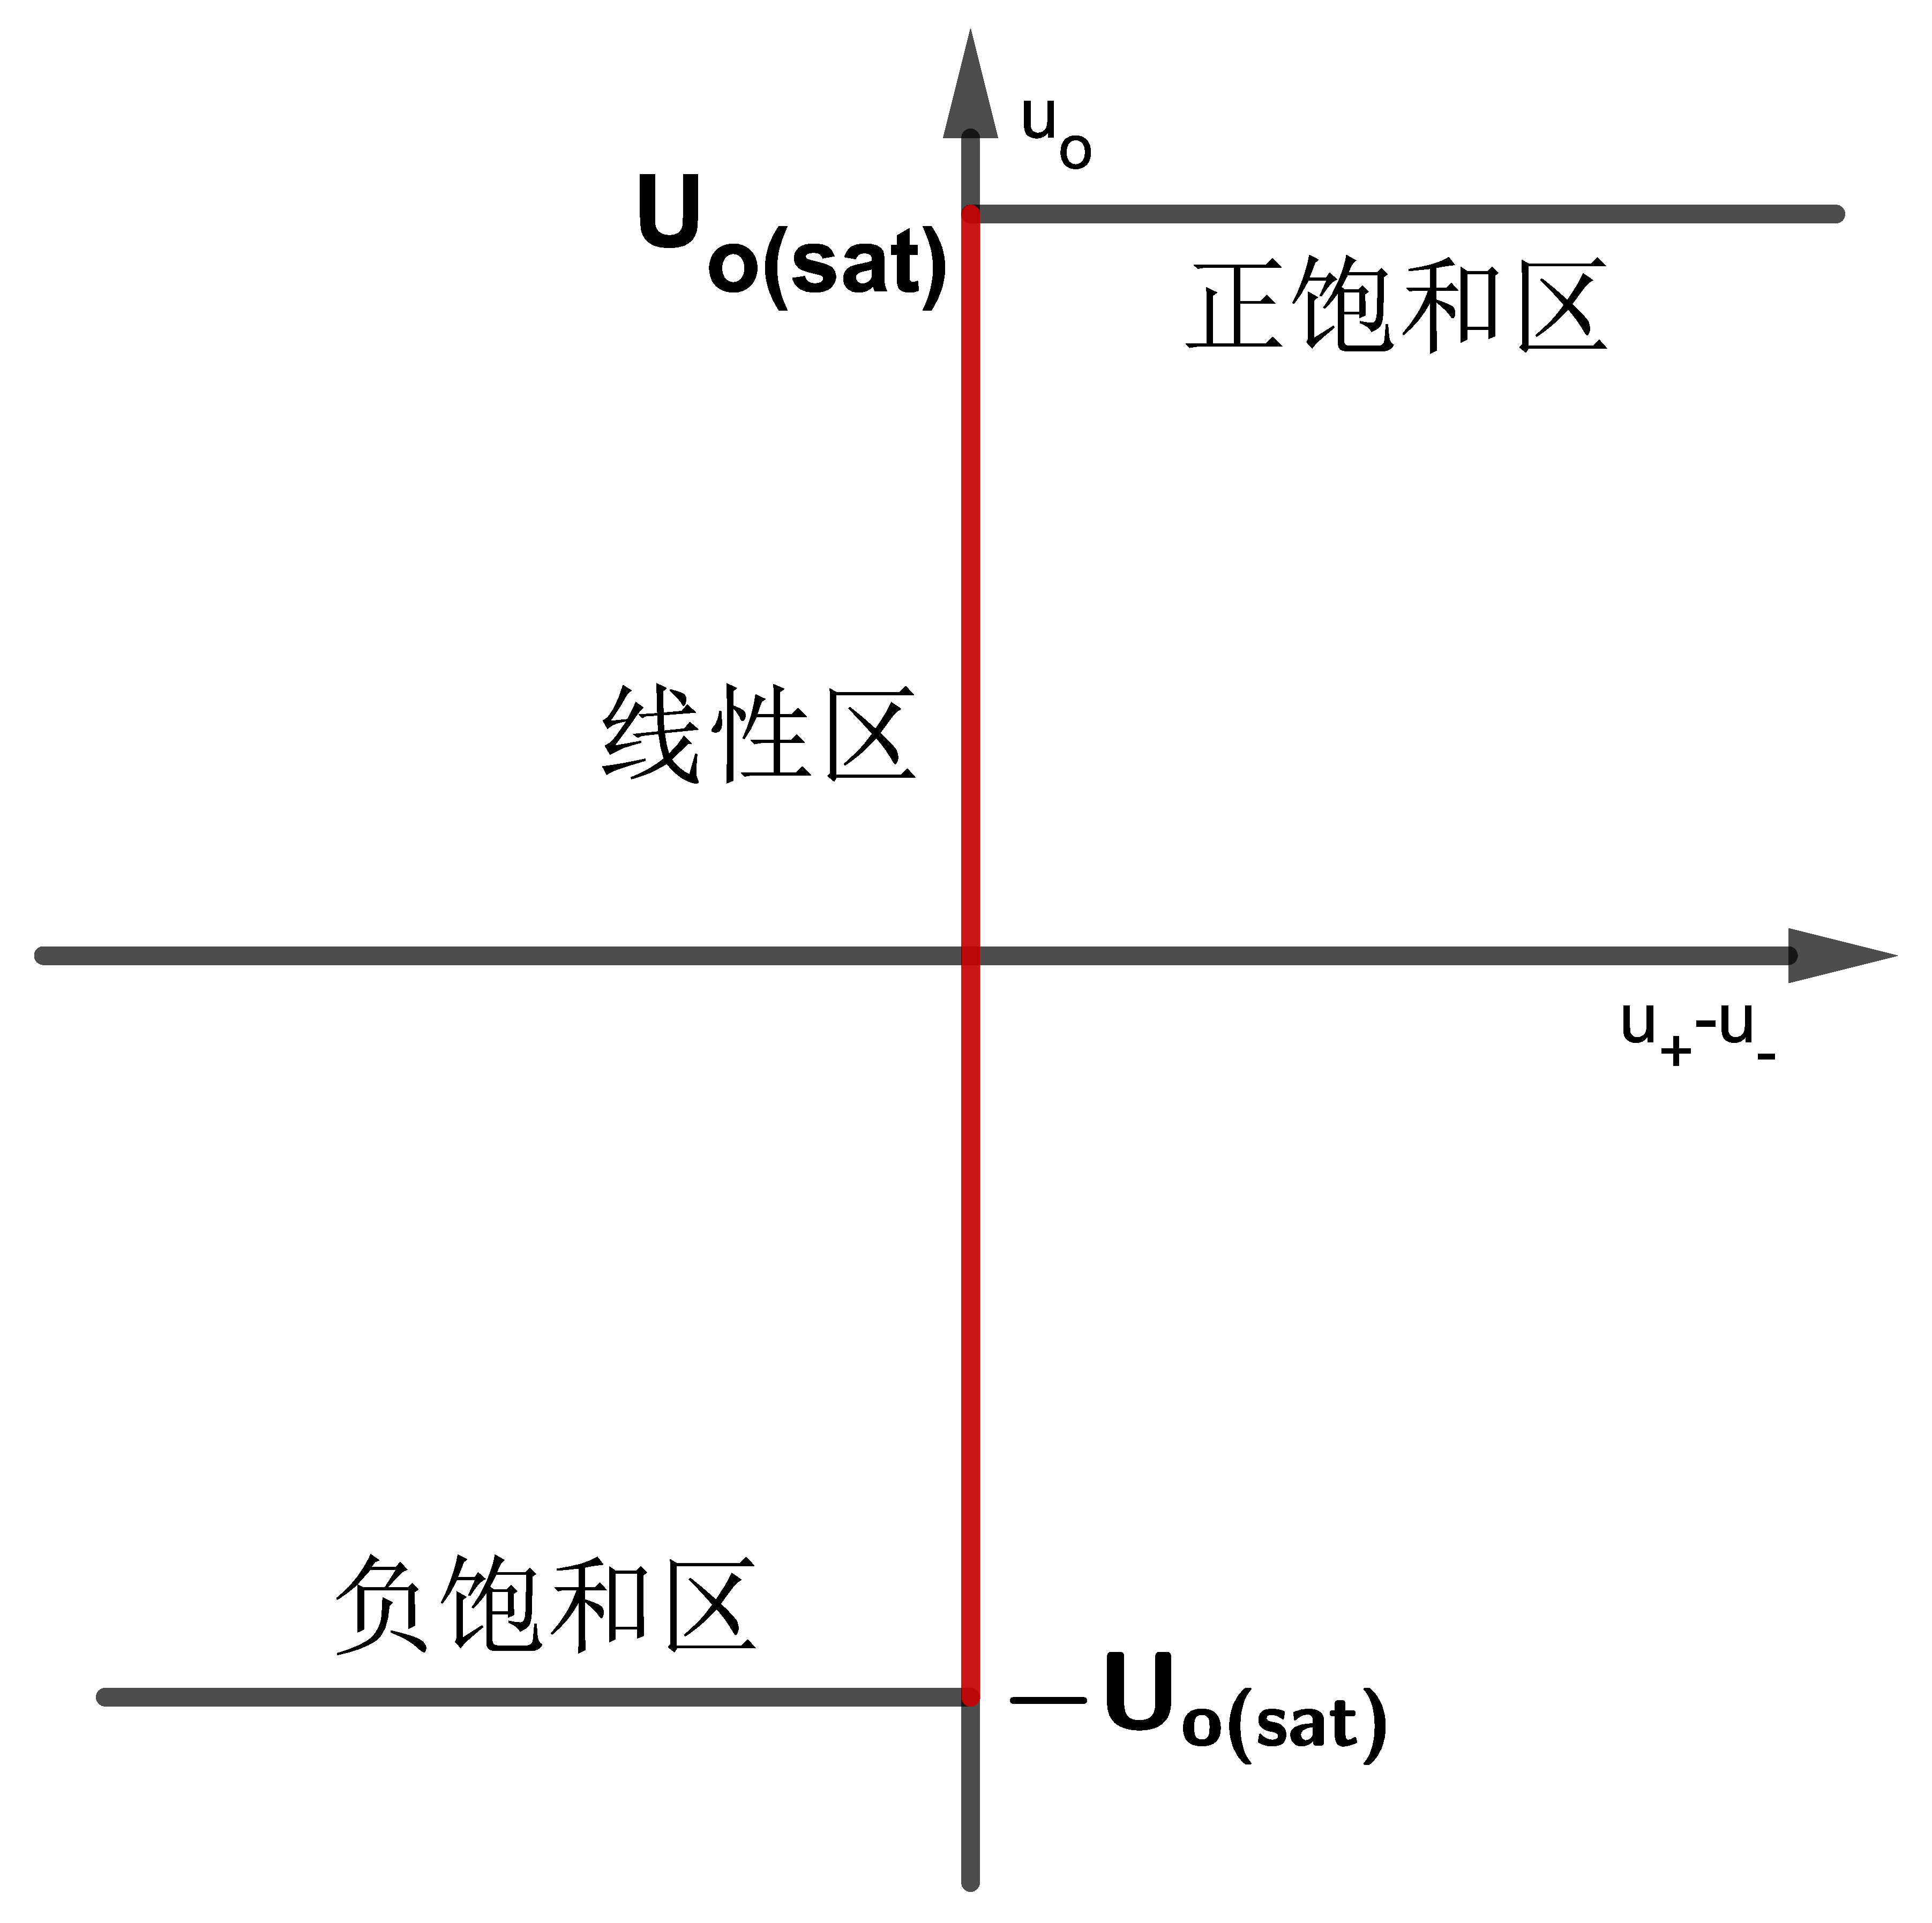
\includegraphics[width=0.35\textwidth]{理想电压传输特性}
	\caption{理想运放的电压传输特性}
	\label{fig:理想运放的电压传输特性}
\end{figure}
\Par 当$u_+=u_-$时,它处于线性区,能够正常放大;当$u_+\ne u_-$时,它处于饱和区.当它处于线性区时,由于$u_+=u_-$,因此它们的电位必然相同,我们称之为\textbf{虚短}.同时,由于输入电阻$\mathrm{r}_{\mathrm{id}}\to \infty$,因此它们没有输入电流,这被称作\textbf{虚断}.而当它处于饱和区时,可以知道,它不存在虚短现象,但是存在虚断状态.